\chapter{Materials and Methods}
\label{chapter:materials_and_methods}

This chapter covers a review of the experimental infrastructure including relevant hardware and software tools used while developing the final solution.

\section{Hardware Setup}

The experimental part of this thesis was developed using the setup available at the Laboratory for Automation and Robotics (LAR) located in the Department of Mechanical Engineering at the University of Aveiro. This setup was designed to meet the requirements of the AUGMANITY mobilizing project\footnote{AUGMANITY website: \url{https://www.augmanity.pt}} and it contains an UR10e collaborative robot and multiple cameras, including the Orbbec Astra Pro RGBD camera which was utilized.

\textcolor{red}{Image of the setup}

\subsection{UR10e Robot}

UR10e is a collaborative robot model developed by Universal Robots focused on versatility. It allows for payloads up to 12.5 kg and has a reach of 1300mm being suitable for tasks such as machine tending, palletizing, and packaging\cite{UR10e}. The one used in this work is equipped with a \textcolor{red}{(missing gripper model)} gripper.

\begin{figure}[h]
\centerline{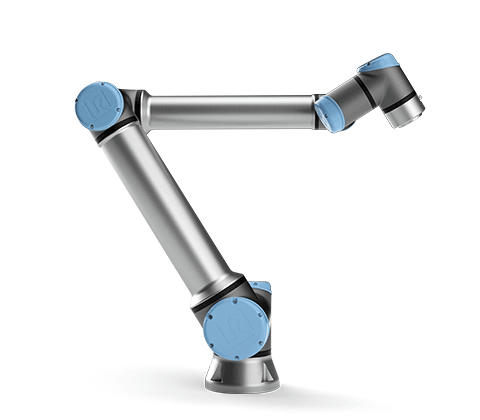
\includegraphics[height=2.5in]{figs/UR10e.png}}
\caption[UR10e]{UR10e collaborative robot \cite{UR10e_image} \textcolor{red}{(missing gripper image)}}
\label{fig:ur10e}
\end{figure}

\subsection{Orbbec Astra Pro}

Orbbec Astra Pro is an RGBD camera developed by Orbbec Technologies. It is frequently used in computer vision and robotics for tasks such as face recognition, gesture recognition, human body tracking, three-dimensional measurement, environment perception, and three-dimensional map reconstruction\cite{AstraPro}. In this work, the camera is placed above the environment facing down capturing both color and depth real-time images.

\begin{figure}[h]
\centerline{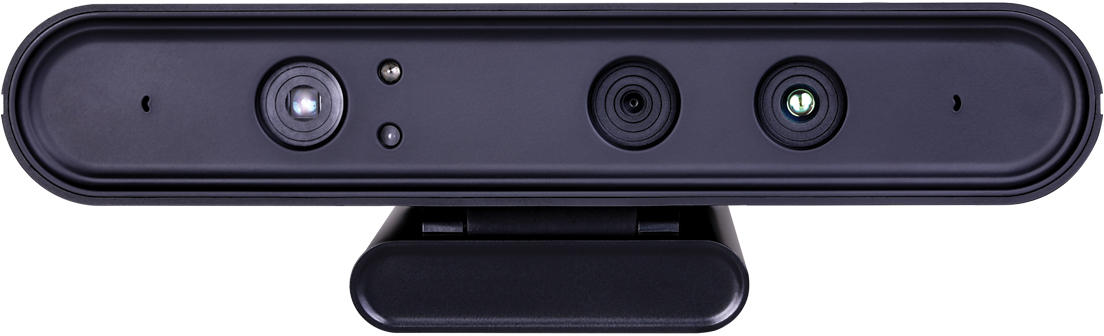
\includegraphics[height=1.2in]{figs/Astra.jpg}}
\caption[Orbbec Astra Pro]{Orbbec Astra Pro \cite{AstraPro}}
\label{fig:orbbec_astra_pro}
\end{figure}

\section{Software Tools}

\subsection{\acf{ros}}

\acs{ros}\cite{ROS2}\footnote{\acs{ros} 1 documentation: \url{https://wiki.ros.org}}\footnote{\acs{ros} 2 documentation: \url{https://docs.ros.org/en/humble}} is an open-source collection of tools and software libraries used to develop a robotics application. Its main features are:

\begin{itemize}
    \item \textbf{message broker}: every process in the project is a node in the \acs{ros} network and communicates with the other nodes mainly through topics (asynchronous publish/subscribe streaming of data) or services (synchronous RPC-style communication);
    \item \textbf{code reuse}: executables and packages are written to be as independent as possible, making the developer able to reuse them in another project;
    \item \textbf{rich ecosystem}: there are several open-source packages available to the developer that can be easily integrated;
    \item \textbf{scalability}: given that the nodes are so loosely coupled, it allows for node distribution;
    \item \textbf{language independence}: nodes can be written in any language since communication is established through well-defined objects;
    \item \textbf{data visualization}: there are tools to visualize the data in real-time, such as Rviz;
    \item \textbf{simulator support}: \acs{ros} has support for simulators with Gazebo being the most common;
    \item \textbf{hardware abstraction}: contains driver packages to deal with some hardware devices;
\end{itemize}

In this work, \acs{ros} is used to establish communication throughout all of the infrastructure. This makes it easier to integrate with previously developed software for the robot and set up the necessary drivers both for the robot and the camera. Additionally, Rviz is used to help visualize the functioning of the system.

\subsection{MoveIt}

MoveIt\footnote{MoveIt documentation: \url{https://ros-planning.github.io/moveit_tutorials}} is a widely-used open-source framework for robotics applications involving motion planning, manipulation, 3D perception, kinematics, control, navigation, and collision checking. MoveIt is implemented on top of ROS taking advantage of the latter's features such as the messaging and build systems as well as standard tools such as ROS Visualizer (Rviz) and the ROS robot format (URDF).

In this work, the MoveIt framework is used to plan and execute the robot arm movements with OMPL, an open-source motion planning library used by MoveIt for motion planning tasks.

\subsection{Tensorflow}

Tensorflow\footnote{Tensorflow documentation: \url{https://www.tensorflow.org/api_docs}} is a platform that can be used for all steps of a machine learning project. Its main features are:
\begin{itemize}
    \item \textbf{prepare data}: load data, data pre-processing and data augmentation;
    \item \textbf{build models}: design and train custom models with little code or use pre-trained ones (transfer learning);
    \item \textbf{deploy models}: helps using models in different platforms such as locally, in the cloud, in a browser, or in mobile;
    \item \textbf{implement MLOps}: run models in production, tracking their performance and identifying issues.
\end{itemize}

In this work, Tensorflow is used to design and train the machine learning models.

\section{Methods}

This section explains the methods used in this work in greater detail.

\subsection{LSTM}

\subsection{Transformer Neural Networks}

Transformer Neural Networks consist of a new kind of neural network architecture that aims to solve tasks involving sequence data such as those in natural language processing. They were initially proposed in the "Attention Is All You Need" paper published by Google Research in 2017\cite{Vaswani2017} and proceeded to surpass several established architectures in numerous tasks using attention mechanisms that identify complex relationships between elements in the input sequence.

According to \textcolor{red}{https://learning.oreilly.com/library/view/deep-learning-with/9781803232911/}, the transformer's architectures are built upon 4 core concepts: positional encoding, attention, self-attention, and multi-head (self-)attention.

\subsubsection{Positional encoding}

RNNs are able to work with sequences given that the tokens are processed sequentially. However, this approach comes with the disadvantage of the model having greater difficulty in analyzing long sequences, since important data might be forgotten. Transformers address this issue by using positional encoding, assigning a unique number to each token representing its position in the input sequence. This enables the transformer to learn the significance of each token's position.

\subsubsection{Attention}

Attention is a concept that consists in measuring the relative importance of the input tokens to the output tokens. It was initially designed to facilitate language translation given that, when translating text from one language to the other, each word in the output can be influenced by multiple words from the input, and it became a key idea behind the transformer's architecture.

\subsubsection{Self-attention}

Self-attention derives from attention but consists in measuring the relative importance of the input tokens to the other tokens of the input sequence instead of the output tokens. This concept allows the model to learn the relationships between tokens and their relevance in the input sequence even if they are far away.
 
\subsubsection{Multi-head (self-)attention}

Multi-head (self-)attention refers to the fact that a transformer can have multiple attention heads. Each attention head performs a parallel process of (self-)attention allowing for multiple resulting weight matrices and, therefore, multiple definitions of relevance between the tokens.

\subsubsection{Architecture}

\begin{figure}[h]
\centerline{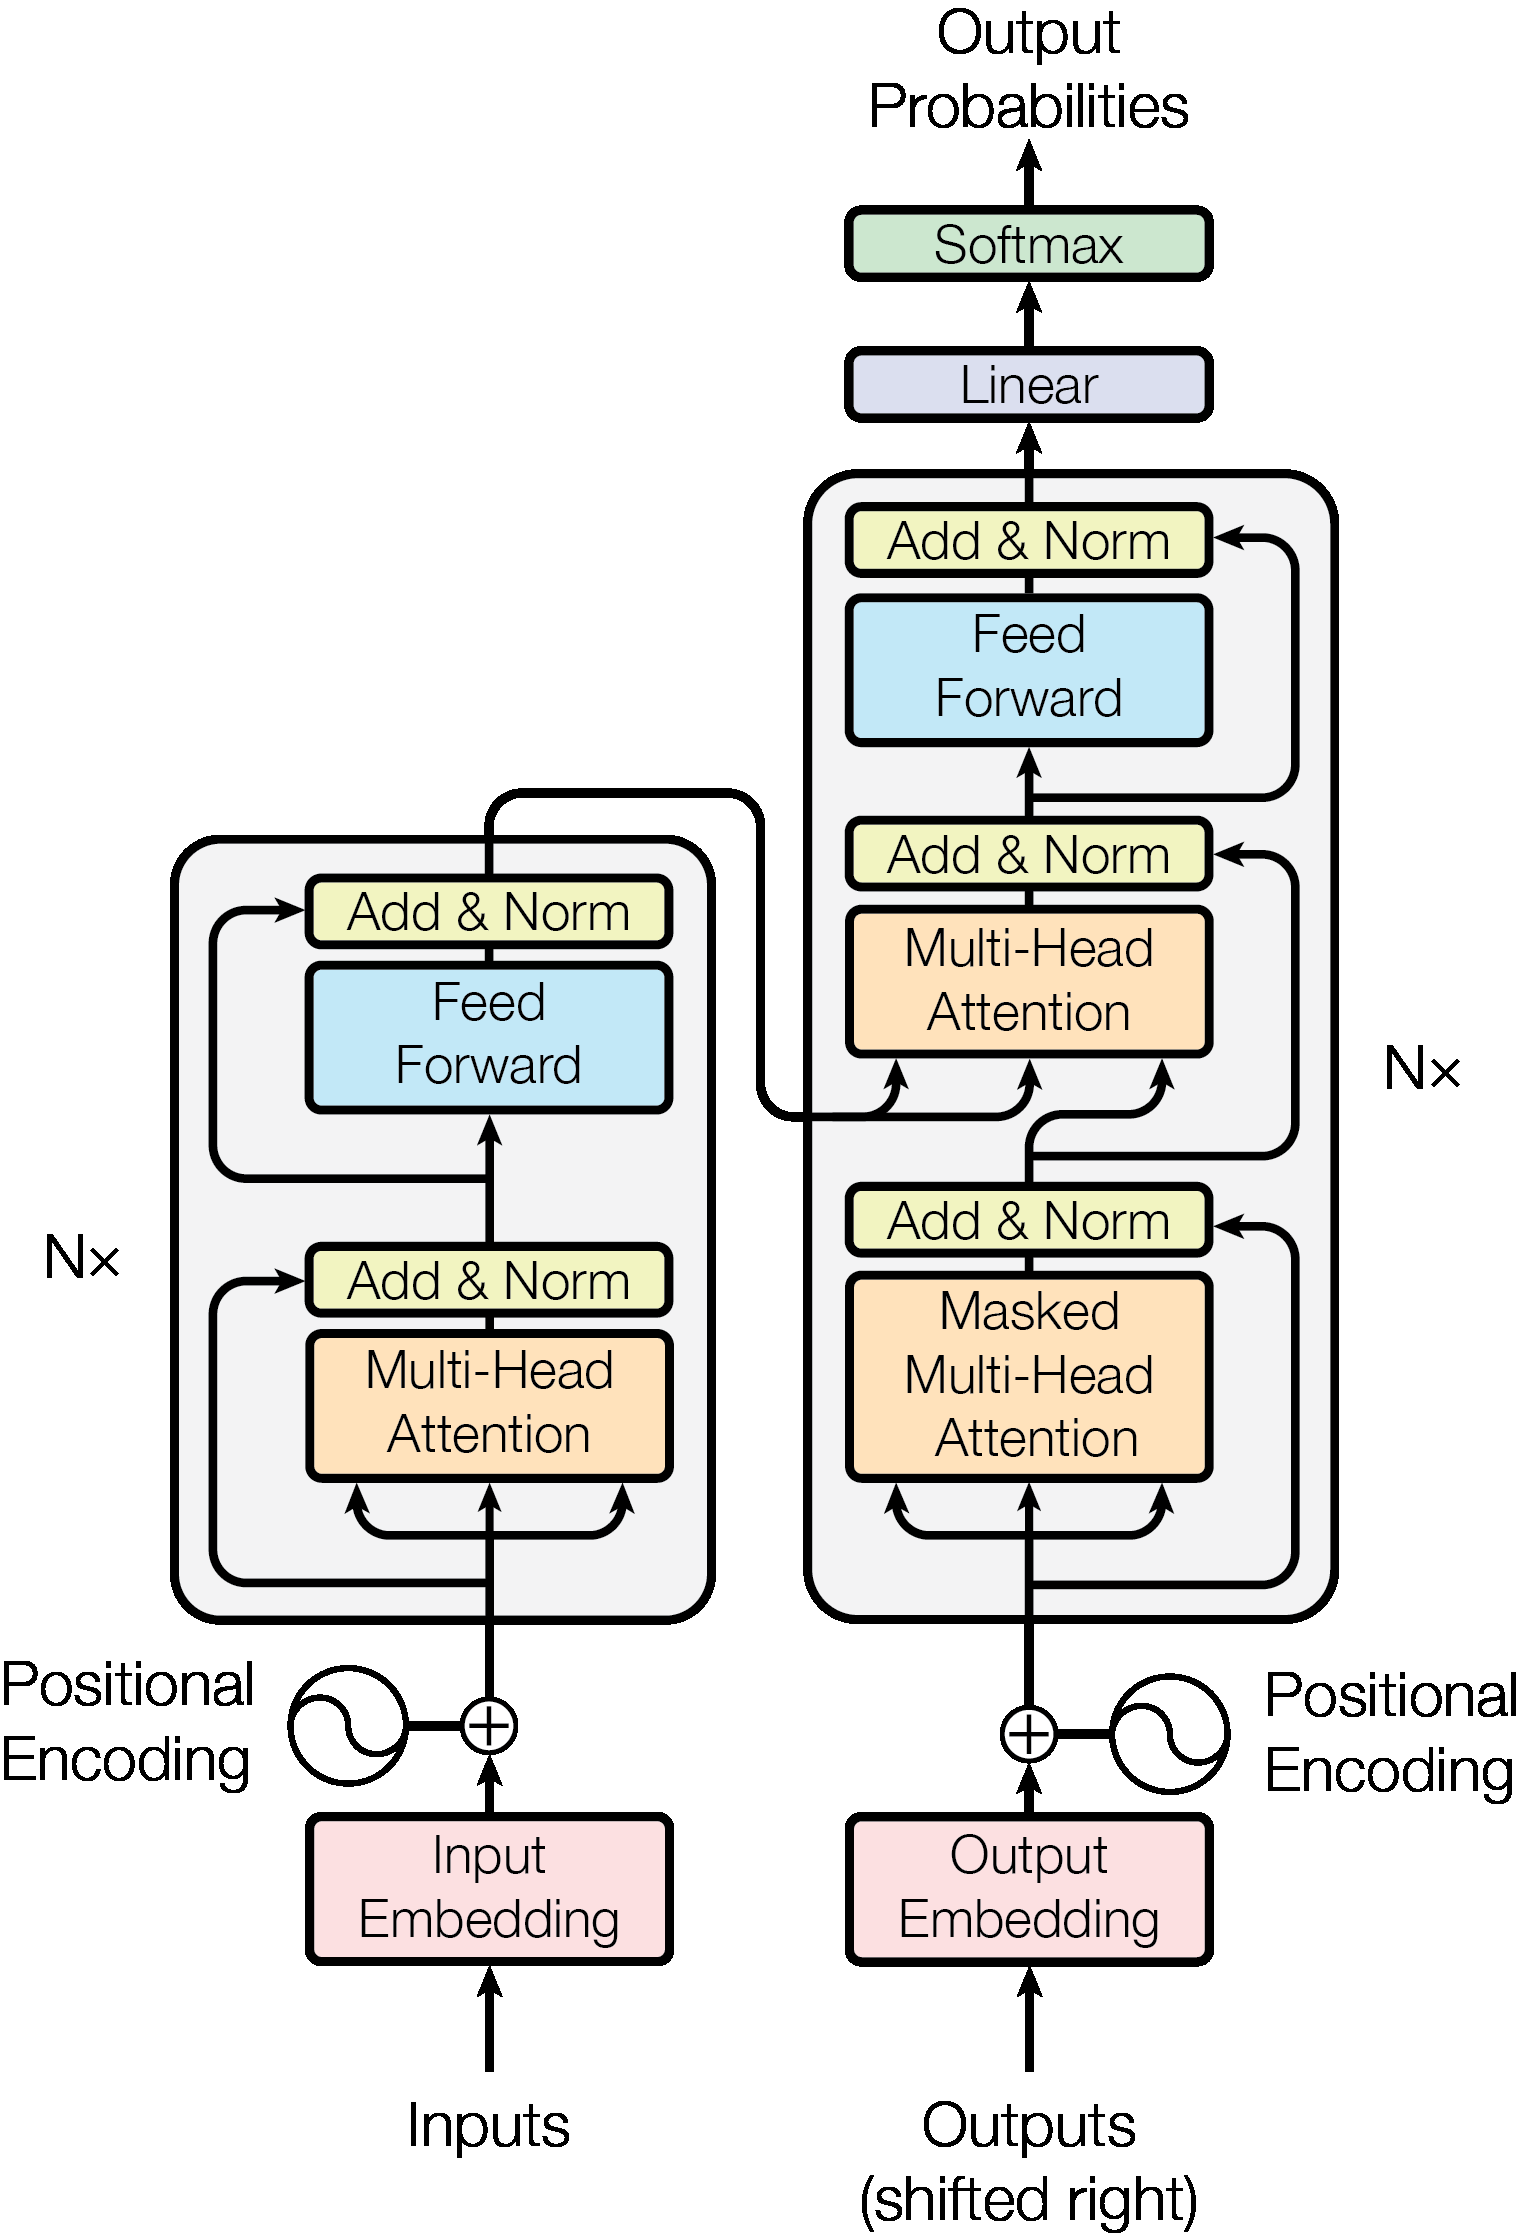
\includegraphics[height=6in]{figs/transformer.jpg}}
\caption[Transformer Architecture]{Transformer Architecture \cite{Vaswani2017}}
\label{fig:transformer_arch}
\end{figure}
